\documentclass[10pt]{article}
\usepackage[margin=1in]{geometry} 
\usepackage{enumerate, xfrac, color, graphicx}
\usepackage{amsmath,amsthm,amssymb,amsfonts,mathabx}
\usepackage{booktabs}
\usepackage{caption}
\usepackage{algorithm}
\usepackage{algpseudocode}
\usepackage{pifont}
\usepackage{listings, courier}
\graphicspath{{/Users/mfzhao/Dropbox/}}
\newcommand{\N}{\mathbb{N}}
\newcommand{\Z}{\mathbb{Z}}
\lstset{breaklines=true, basicstyle=\small\ttfamily, language=R, backgroundcolor=\color{highlight}, stepnumber=5}

\definecolor{highlight}{RGB}{248,248,248}

\begin{document}
	\title{6.867 Problem Set 3}
	\maketitle
	
\subsubsection*{Neural Networks}

In some cases, we might want to use a neural network rather than another algorithm, such as SVM or logistic regression, in order to be somewhat more agnostic about the parametric form of the data-generating process. In this case, we investigate the use of neural networks, first on some toy training data sets, and subsequently on a subset of the popular MNIST dataset.

Let us first briefly review the way that neural network works. Neural networks are inspired by how brains process information. In the brain we have interconnected neurons that produce electrochemical impulses that feed into other neurons. In a neural network, we try to mimic this architecture by using interconnected ``perceptrons`` or nodes. These nodes are organized into ``layers`` which are connected to nodes in other layers, but not to nodes in the same layer. 

In a feed-forward neural network (the specific type of neural network architecture we are working with). The outputs of each layer are fully connected to the next layer. These layer to layer connections are represented by a weight matrix. Functionally, the weight matrix produces a weighted linear combination of the outputs of a layer to use as the input for the next layer. This weighted linear combination is then fed into some nonlinear ``activation function`` on each node (typically a sigmoid function or tanh function) which produces the output of a node. Its important to note that the activation function needs to be nonlinear otherwise we would end up with a standard linear model (a linear combination of linear function is still a linear function). These outputs can then be fed into a new layer via the same procedure as above. We can arbitrarily choose how many of these interconnected layers we want to include in a neural network model. 

\begin{figure}[ht]
	\centering
	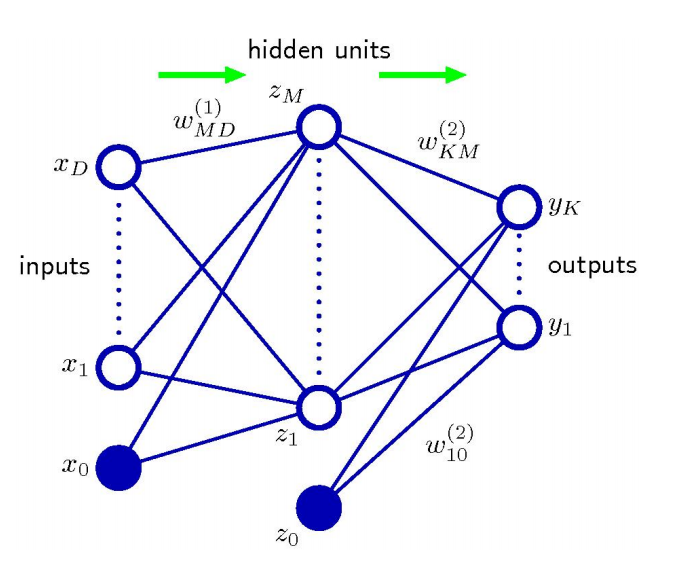
\includegraphics[height=3in]{neuralnetdiagram.png}
	\caption*{Figure 1: A schematic diagram of a neural network (taken from the homework assignment document)}
\end{figure}

However, a neural network model needs at the very least two layers, an input layer and an output layer. These layers are our data, where the input layer is composed of our features and the output layer is what we want to predict. In this sense, the simplest neural network  with a single node in the output layer is just a logistic regression. For networks with more than just the input layer and output layer, the intermediate layers are called ``hidden layers`` since they're not directly observed but are learned (much like a hidden state in a Hidden Markov Model). A schematic sketch of a neural net with a single hidden layer can be found above. Alternatively, this neural network may be mathematically specified as follows:

\begin{equation}
a_{n}^{(1)} = \sum_d w_{dn}^{(1)}x_d
\end{equation}

\begin{equation}
z_{n}^{(1)} = f_1(a_n^{(1)})
\end{equation}

\begin{equation}
a_{k}^{(2)} = \sum_k w_{nk}^{(2)}z_n
\end{equation}

\begin{equation}
y_k = z_{k}^{(2)} = f_2(a_k^{(2)})
\end{equation}

Or in matrix notation:
\begin{equation}
a^{(1)} = X\cdot W^{(1)}	
\end{equation}

\begin{equation}
z^{(1)} = f_1(a^{(1)})
\end{equation}

\begin{equation}
a^{(2)} = z^{(1)}\cdot W^{(2)}	
\end{equation}

\begin{equation}
y = z^{(2)} = f_1(a^{(2)})
\end{equation}

For the purposes of this paper, we will try to solve simple multi-class prediction problems using a neural network with one hidden layer. In order to determine the weight matrices that give us the best predictive accuracy, we will specify a loss function and perform (batch or stochastic) gradient descent. We specify our objective function as the regularized negative log-likelihood function:

\begin{equation}
J(w) = l(w) +\lambda(||w^{(1)}||^2_F + ||w^{(2)}||^2_F
\end{equation}

\noindent where $l(w)$ is

\begin{equation}
l(w) = \sum_{i=1}^N \sum_{k=1}^{K} [-y_k^{(i)}\log(h_k(x^{(i)},w)) - (1-y_k^{(i)})\log(1-(h_k(x^{(i)},w))].
\end{equation}

In order to calculate the gradient as a function of $w_1$ and $w_2$, we use the two gradient calculation expressions below:

\begin{equation}
\frac{\partial J(w)}{\partial w_{kj}^{(2)}} = \sum_{i=1}^N z_j \left(\sigma(a_k^{(2)}) -y_k^{(i)} \right) + 2 \lambda w_{kj}^{(2)}
\end{equation}

\noindent and 

\begin{equation}
\frac{\partial J(w)}{\partial w_{jd}^{(1)}} =  \sum_{i=1}^N x_i \sum_{k=1}^{K} \left(\sigma(a_k^{(2)}) -y_k^{(i)}\right) w_{kj}^{(2)} \left(\sigma(a_{jd}^{(1)})\right)\left(1-\sigma(a_{jd}^{(1)})\right) + 2 \lambda w_{jd}^{(1)}.
\end{equation}

Let's now see how a neural network performs on two different toy data sets. We vary both the number of hidden nodes and the regularization parameter in our objective function, and use both full gradient descent and mini-batch stochastic gradient descent (with a batch size of 10). In particular, we use mini-batch SGD as opposed to full SGD (where batch size is 1) since mini-batch generally has better convergence properties. The two algorithms perform comparably - in the case of toy data set number 2, we find that the full gradient descent algorithm does a slightly better job at finding the optimal values of our parameter than stochastic gradient descent (classification error of 6.7\% as opposed to 9\%). While full gradient descent does perform better, its important to note the SGD was significantly faster. This should be expected since full-batch uses the entire dataset to perform an update while SGD only uses a fraction, meaning that when we use SGD as opposed to full gradient descent we lose some of the nice convergence properties to gain faster updates. 

It's important to note that our changes in parameters have a much larger effect on the performance for toy dataset 2 than for our features in toy dataset 1. This is likely due to the lack of an easy way to separate examples of different classes in dataset 2.

\begin{figure}[ht]
	\centering
	\begin{minipage}[b]{.48\linewidth}
		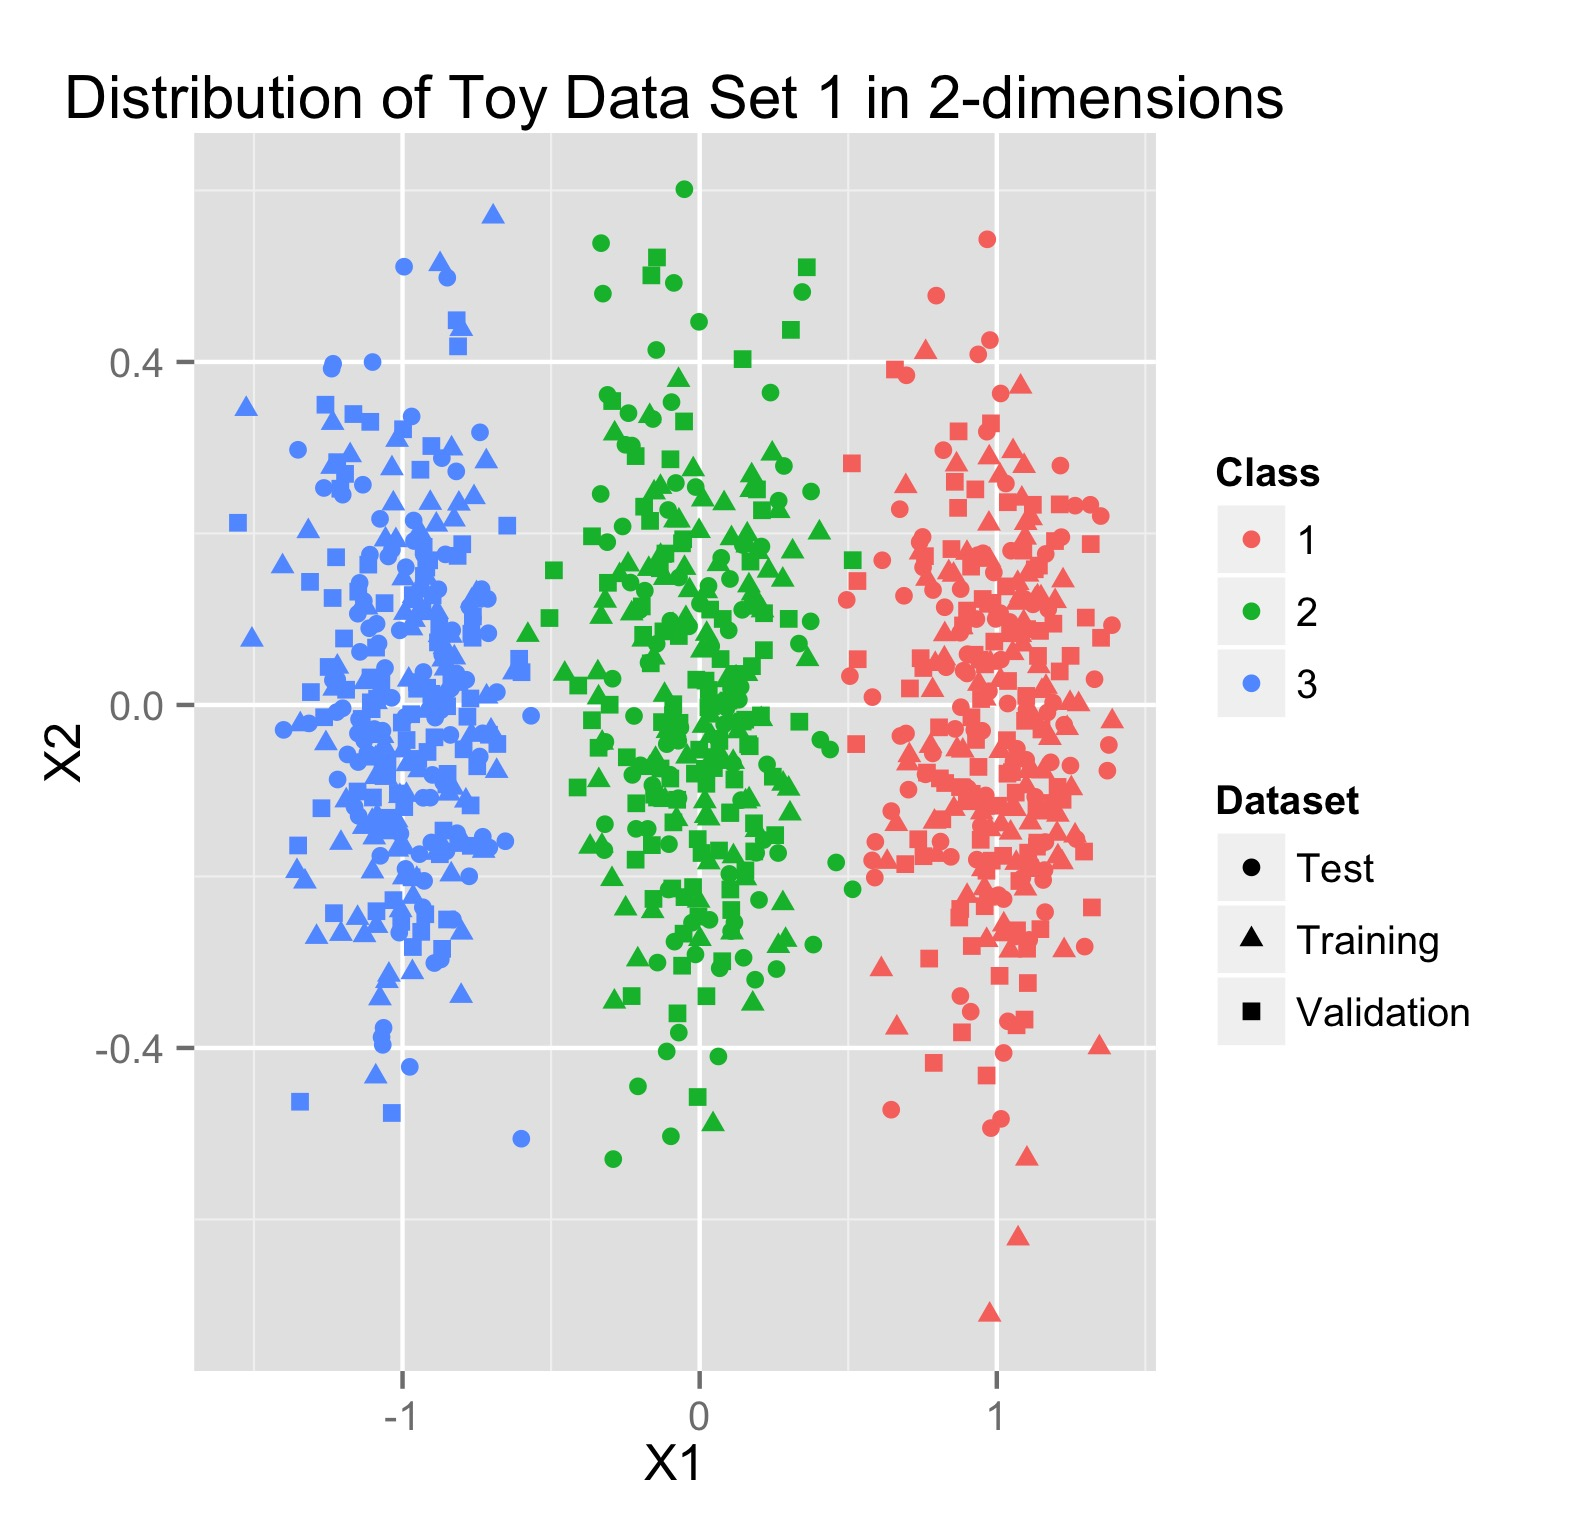
\includegraphics[width=1\linewidth, height=2.7in]{t1dist.jpg}
		\caption*{Toy Dataset \#1}
	\end{minipage}
	\begin{minipage}[b]{.48\linewidth}
		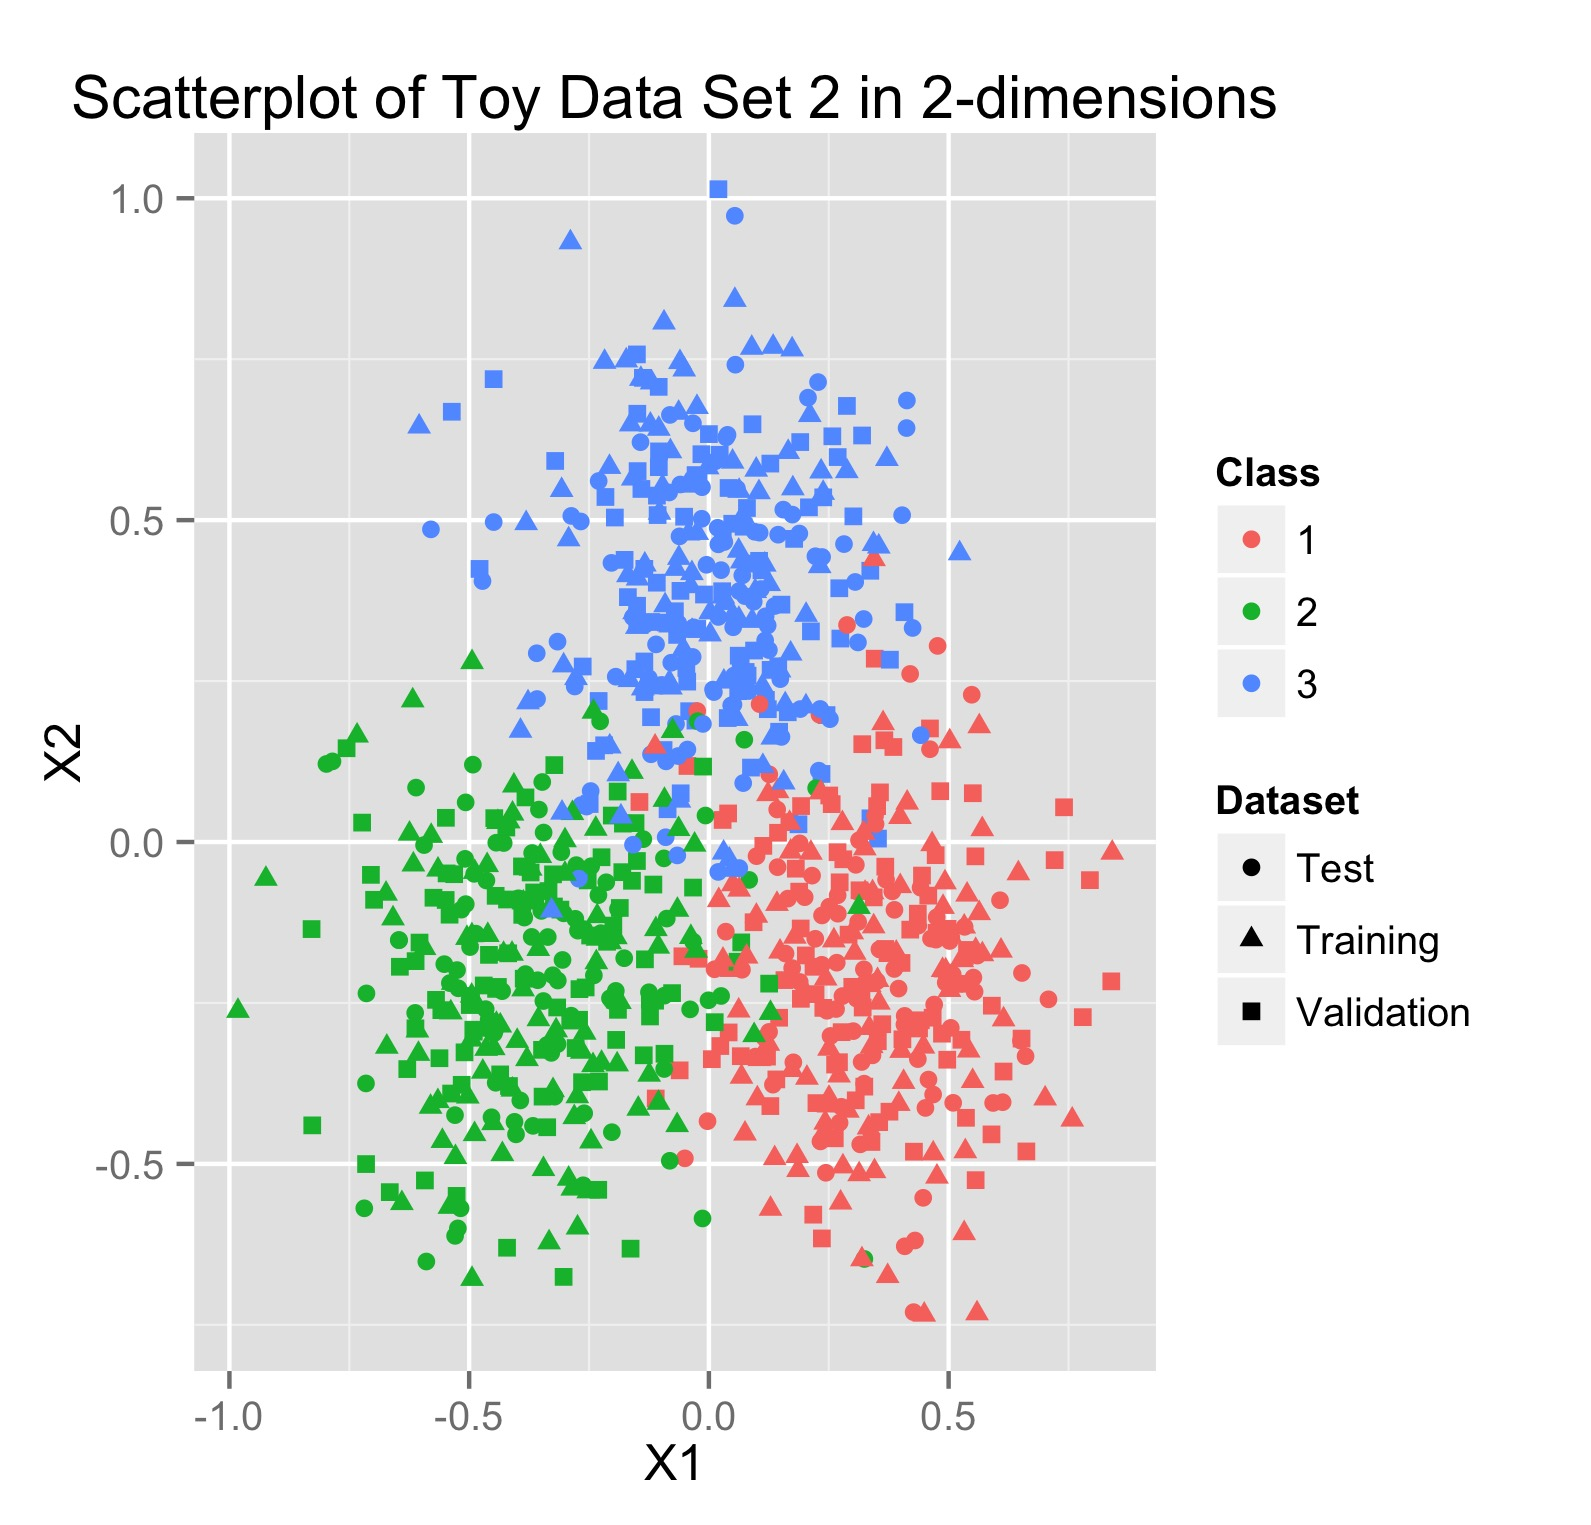
\includegraphics[width=1\linewidth, height=2.7in]{t2dist.jpg}
		\caption*{Toy Dataset \#2}
	\end{minipage}
	\caption{Distributions of different classes in $X1$, $X2$ for toy datasets}
\end{figure}

\begin{table}
\captionof{table}{Performance of neural network with full gradient descent on Toy Data Set 1 (training)} 
\centering
\begin{tabular}{llllll}
\toprule
& $n_1$ = \bf{1} & $n_1$ =  \bf{3} & $n_1$ =  \bf{5} & $n_1$ =  \bf{7} & $n_1$ =  \bf{9} \\
\midrule
$\lambda$ = \bf{0} &  0.007 & \bf{0}     & 0     & 0     & 0     \\
$\lambda$ = \bf{1e-5} & 0.007 & 0     & 0     & 0     & 0     \\
$\lambda$ = \bf{1e-3} & 0.093 & 0.003 & 0.003 & 0.003 & 0.003 \\
$\lambda$ = \bf{1e-1} & 0.667 & 0.667 & 0.667 & 0.667 & 0.667 \\
\bottomrule
\end{tabular}
\end{table}

\begin{table}
\captionof{table}{Performance of neural network with full gradient descent on Toy Data Set 1 (validation)} 
\centering
\begin{tabular}{llllll}
\toprule
& $n_1$ = \bf{1} & $n_1$ =  \bf{3} & $n_1$ =  \bf{5} & $n_1$ =  \bf{7} & $n_1$ =  \bf{9} \\
\midrule
$\lambda$ = \bf{0} &      0.01  & \bf{0.003} & 0.003 & 0.003 & 0.003 \\
$\lambda$ = \bf{1e-5} &  0.01  & 0.003 & 0.003 & 0.003 & 0.003 \\
$\lambda$ = \bf{1e-3} &  0.063 & 0.003 & 0.003 & 0.003 & 0.007 \\
$\lambda$ = \bf{1e-1} &  0.667 & 0.667 & 0.667 & 0.667 & 0.667 \\
\bottomrule
\end{tabular}
\end{table}

\begin{table}
\captionof{table}{Performance of neural network with stochastic gradient descent on Toy Data Set 1 (training)} 
\centering
\begin{tabular}{llllll}
\toprule
& $n_1$ = \bf{1} & $n_1$ =  \bf{3} & $n_1$ =  \bf{5} & $n_1$ =  \bf{7} & $n_1$ =  \bf{9} \\
\midrule
$\lambda$ = \bf{0} &       \bf{0.003} & 0.003 & 0.003 & 0.003 & 0.003 \\
$\lambda$ = \bf{1e-5} &   0.043 & 0     & 0.003 & 0.003 & 0     \\
$\lambda$ = \bf{1e-3} &   0.117 & 0     & 0.003 & 0.003 & 0.003 \\
$\lambda$ = \bf{1e-1} &   0.667 & 0.667 & 0.667 & 0.667 & 0.667 \\
\bottomrule
\end{tabular}
\end{table}
	
\begin{table}
\captionof{table}{Performance of neural network with stochastic gradient descent on Toy Data Set 1 (validation)} 
\centering
\begin{tabular}{llllll}
\toprule
& $n_1$ = \bf{1} & $n_1$ =  \bf{3} & $n_1$ =  \bf{5} & $n_1$ =  \bf{7} & $n_1$ =  \bf{9} \\
\midrule
$\lambda$ = \bf{0} &        \bf{0.003} & 0.003 & 0.01  & 0.007 & 0.003 \\
$\lambda$ = \bf{1e-5} &    0.033 & 0.007 & 0.003 & 0.007 & 0.003 \\
$\lambda$ = \bf{1e-3} &    0.097 & 0.013 & 0.013 & 0.013 & 0.013 \\
$\lambda$ = \bf{1e-1} &    0.667 & 0.667 & 0.667 & 0.667 & 0.667 \\
\bottomrule
\end{tabular}
\end{table}


\begin{table}
\captionof{table}{Performance of neural network with full gradient descent on Toy Data Set 2 (training)} 
\centering
\begin{tabular}{llllll}
\toprule
& $n_1$ = \bf{1} & $n_1$ =  \bf{3} & $n_1$ =  \bf{5} & $n_1$ =  \bf{7} & $n_1$ =  \bf{9} \\
\midrule
$\lambda$ = \bf{0} &  0.36  & 0.063 & 0.047 & 0.05  & 0.027 \\
$\lambda$ = \bf{1e-5} & 0.397 & 0.063 & 0.067 & 0.063 & 0.067 \\
$\lambda$ = \bf{1e-3} & 0.413 & \bf{0.06}  & 0.06  & 0.06  & 0.06  \\
$\lambda$ = \bf{1e-1} & 0.667 & 0.667 & 0.667 & 0.667 & 0.667 \\
\bottomrule
\end{tabular}
\end{table}

\begin{table}
\captionof{table}{Performance of neural network with full gradient descent on Toy Data Set 2 (validation)} 
\centering
\begin{tabular}{llllll}
\toprule
& $n_1$ = \bf{1} & $n_1$ =  \bf{3} & $n_1$ =  \bf{5} & $n_1$ =  \bf{7} & $n_1$ =  \bf{9} \\
\midrule
$\lambda$ = \bf{0} &      0.343 & 0.07  & 0.093 & 0.1   & 0.107 \\
$\lambda$ = \bf{1e-5} &   0.39  & 0.073 & 0.07  & 0.073 & 0.073 \\
$\lambda$ = \bf{1e-3} &  0.38  & \bf{0.067} & 0.067 & 0.067 & 0.067 \\
$\lambda$ = \bf{1e-1} &  0.667 & 0.667 & 0.667 & 0.667 & 0.667 \\
\bottomrule
\end{tabular}
\end{table}

\begin{table}
\captionof{table}{Performance of neural network with stochastic gradient descent on Toy Data Set 2 (training)} 
\centering
\begin{tabular}{llllll}
\toprule
& $n_1$ = \bf{1} & $n_1$ =  \bf{3} & $n_1$ =  \bf{5} & $n_1$ =  \bf{7} & $n_1$ =  \bf{9} \\
\midrule
$\lambda$ = \bf{0} &       0.363 & 0.073 & 0.053 & 0.05  & 0.06  \\
$\lambda$ = \bf{1e-5} &   0.363 & 0.07  & \bf{0.067} & 0.057 & 0.067 \\
$\lambda$ = \bf{1e-3} &   0.363 & 0.07  & 0.07  & 0.07  & 0.07  \\
$\lambda$ = \bf{1e-1} &   0.667 & 0.667 & 0.667 & 0.667 & 0.667 \\
\bottomrule
\end{tabular}
\end{table}
	
\begin{table}
\captionof{table}{Performance of neural network with stochastic gradient descent on Toy Data Set 2 (validation)} 
\centering
\begin{tabular}{llllll}
\toprule
& $n_1$ = \bf{1} & $n_1$ =  \bf{3} & $n_1$ =  \bf{5} & $n_1$ =  \bf{7} & $n_1$ =  \bf{9} \\
\midrule
$\lambda$ = \bf{0} &        0.373 & 0.083 & 0.11  & 0.103 & 0.113 \\
$\lambda$ = \bf{1e-5} &    0.373 & 0.087 & \bf{0.077} & 0.08  & 0.09  \\
$\lambda$ = \bf{1e-3} &    0.377 & 0.097 & 0.097 & 0.093 & 0.093 \\
$\lambda$ = \bf{1e-1} &    0.667 & 0.667 & 0.667 & 0.667 & 0.667 \\
\bottomrule
\end{tabular}
\end{table}

We are now interested in testing out neural network code on a real dataset. In our case, we're using a subset the very popular MNIST data collected by Yann Lecunn. This dataset is comprised of 28 by 28 pixel images of handwritten digits with corresponding labels that represent what numbers these images actually represent. For our features, each 28x28 images into a feature vector of 784 where each of these features represent the darkness of a pixel (0 means that its a white pixel, 1 means its a black pixel, everything in between are shades of grey).

When training 


	
\end{document}